\chapter{Resultados Obtidos}

\section{Iteração 1}

\subsection{Engrena}

\subsubsection{Métricas Coletadas}

\begin{itemize}
\item Tamanho do processo:

Foram identificadas um total de \textbf{17 atividades} no processo.

\item Tamanho da equipe:

A equipe é composta por \textbf{4 Membros}.

\item Tamanho do Modelo de Maturidade no processo

Tendo em vista a análise do processo do grupo com o contexto sobre a Engrena, com o olhar voltado na busca por atividades do Mps-Br, foram encontradas um total de \textbf{12 atividades} previstas no modelo de maturidade, sendo elas:
    \begin{enumerate}
    \item DRE-01: Identificar caracteristicas do produto; levantar RF  e RNF, Entender contexto da empresa; identificar solicitação dos stkeholders.
    \item DRE-02: Produzir plano de iteração.
    \item DRE-03: Elaborar especificação suplementar.
    \item DRE-04: Refinar casos de uso priorizaos; Identificar casos de uso.
    \item DRE-05: Modelar casos de uso.
    \item DRE-06: Modelar casos de uso.
    \item DRE-07: Levantar RF e RNF.
    \item GRE-01: Identificar caracteristicas do produto; Levantar RF e RNF.
    \item GRE-02: Refinar casos de uso priorizaos; Elaborar especificação suplementar.
    \end{enumerate}

\item Esforço da equipe

\begin{figure}[H]
  \center
  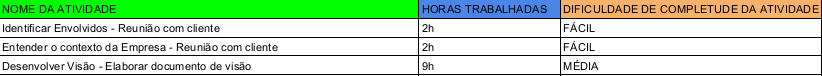
\includegraphics[width=0.8\textwidth]{figuras/esforco-eqp}
  \caption{Esforço da Equipe}
  \label{fig:esforco-eqp}
\end{figure}

\item Esforço dos Monitores

O monitor dedicou-se um total de \textbf{4 horas} nesta iteração em questão.

\item Custo das atividades

Identificar envolvidos: R\$ 61,20

Entender o contexto da empresa: R\$ 61,20

Desenvolver Visão: R\$ 550,8

\item Custo de adesão do modelo de maturidade

DRE-01: R\$ 122,40

\end{itemize}

\subsubsection{Indicadores}

Os indicadores que visamos analisar, para levar em consideração as métricas coletadas são:
\begin{itemize}
\item Satisfação do cliente com os requisitos
\item Satisfação do cliente com o processo
\end{itemize}

Para responder tais, foi elaborado um questionário (figura~\ref{fig:quest1}) e aplicado aos clientes, visando analisar sua satisfação de acordo com os indicadores apresentados acima.

\begin{figure}[H]
  \center
  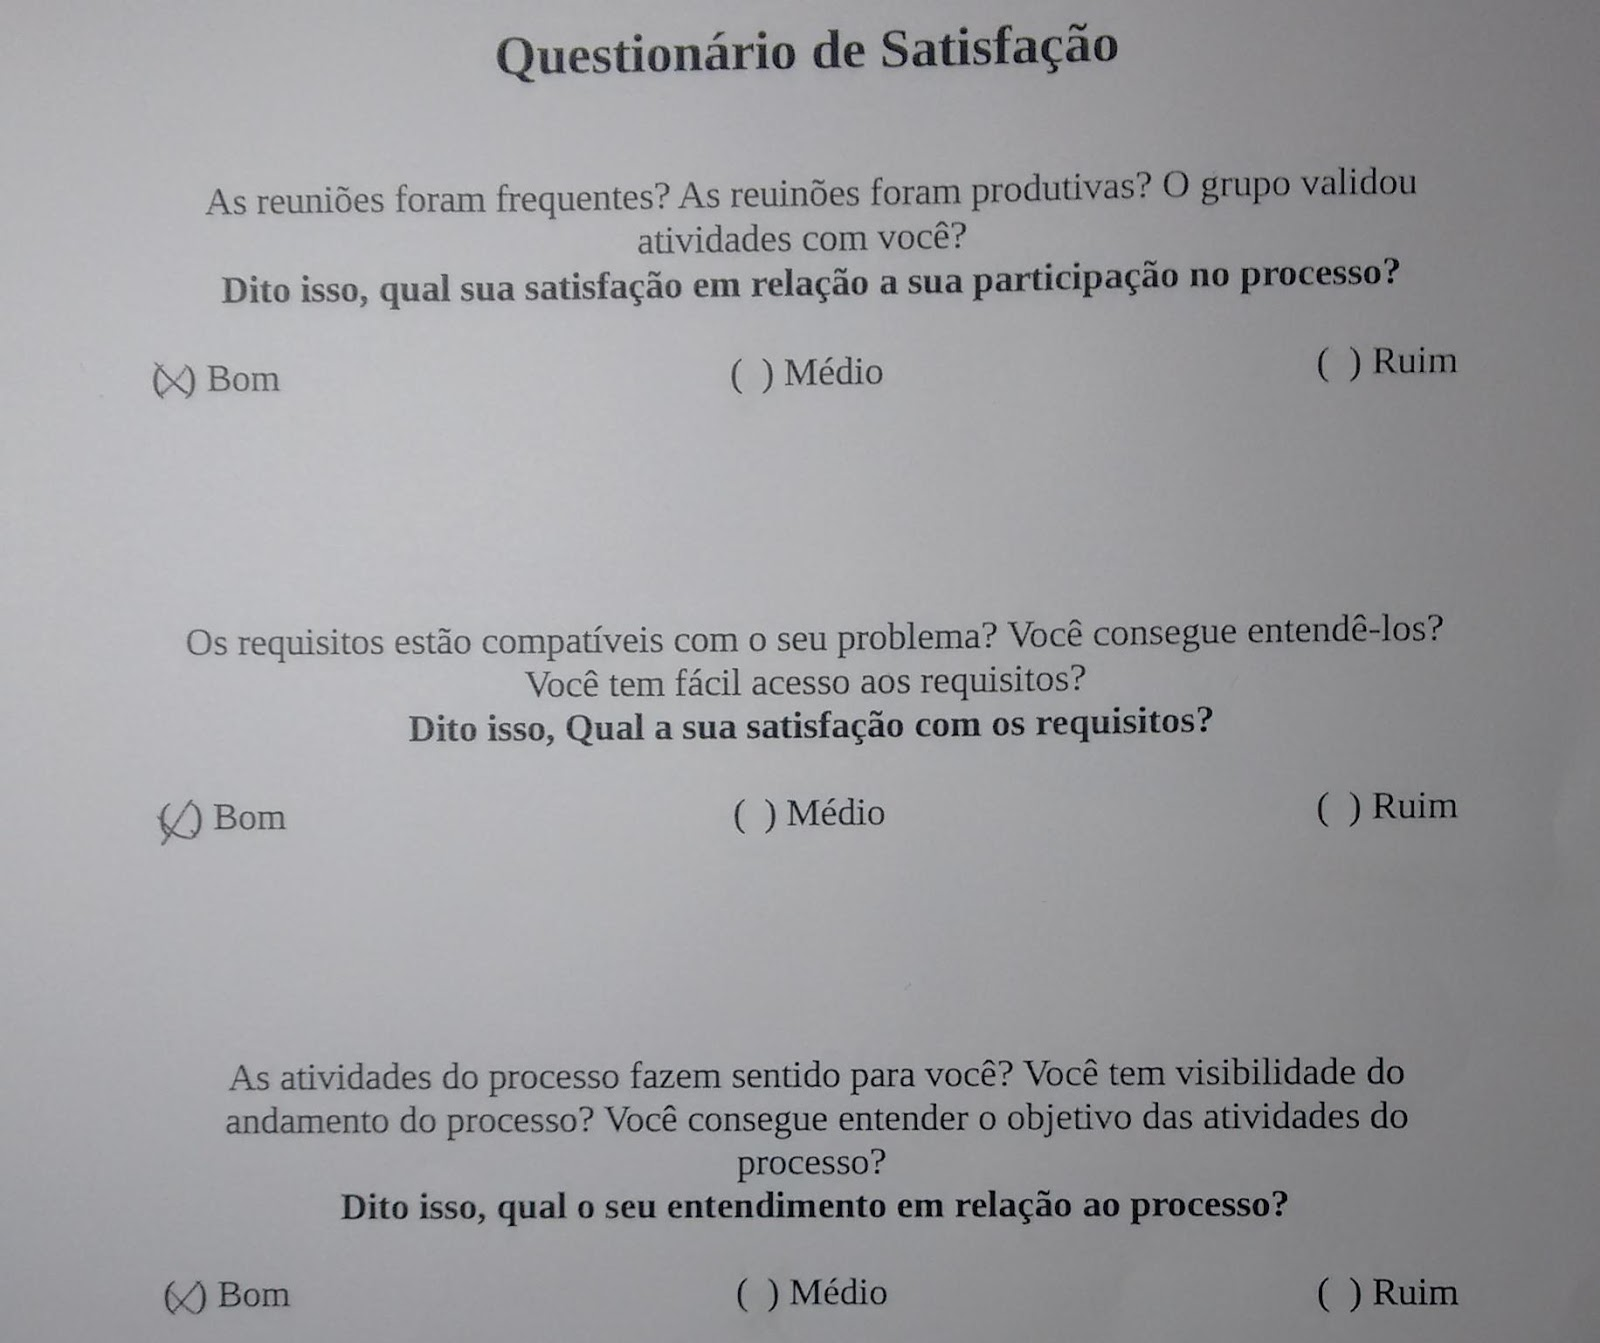
\includegraphics[width=0.8\textwidth]{figuras/quest1}
  \caption{Questionário 1 - Engrena}
  \label{fig:quest1}
\end{figure}

\subsection{Eletrojun}

\begin{itemize}
\item Tamanho do processo:

Foram identificadas um total de \textbf{20 atividades} no processo.

\item Tamanho da equipe:

A equipe é composta por \textbf{3 Membros}.

\item Tamanho do Modelo de Maturidade no processo

Tendo em vista a análise do processo do grupo com o contexto sobre a Engrena, com o olhar voltado na busca por atividades do Mps-Br, foram encontradas um total de \textbf{09 atividades} previstas no modelo de maturidade, sendo elas:

    \begin{enumerate}
    \item DRE-01: Entender contexto da empresa; Identificar solicitação dos stkeholders.
    \item DRE-03: Elaborar especificação suplementar.
    \item DRE-05: Estruturar modelo de caso de uso.
    \item DRE-06: Estruturar modelo de caso de uso.
    \item DRE-08: Validar modelo de caso de uso.
    \item GRE-01: Identificar solicitação dos stkeholders.
    \item GRE-02: Elaborar especificação suplementar.
    \item GRE-04: Implementar mudanças; Melhorar atualizar artefatos.
    \item GRE-05: Analisar impacto das mudanças; Analisar viabilidade das mudanças; Implementar mudanças; Melhorar atualizar artefatos.
    \end{enumerate}

\item Esforço da equipe

O esforço não pode ser coletado na iteração, pois o grupo não havia iniciado as atividades previstas. Logo, não houve nenhum esforço.

\item Esforço dos Monitores

O monitor dedicou-se um total de \textbf{4 horas} nesta iteração em questão.

\item Custo das atividades

R\$ 00,00

\item Custo de adesão do modelo de maturidade

R\$ 00,00

\end{itemize}

\subsubsection{Indicadores}

Os indicadores que visamos analisar, para levar em consideração as métricas coletadas são:
\begin{itemize}
\item Satisfação do cliente com os requisitos
\item Satisfação do cliente com o processo
\end{itemize}

Para responder tais, foi elaborado um questionário (figura~\ref{}) e aplicado aos clientes, visando analisar sua satisfação de acordo com os indicadores apresentados acima.

\begin{figure}[H]
  \center
  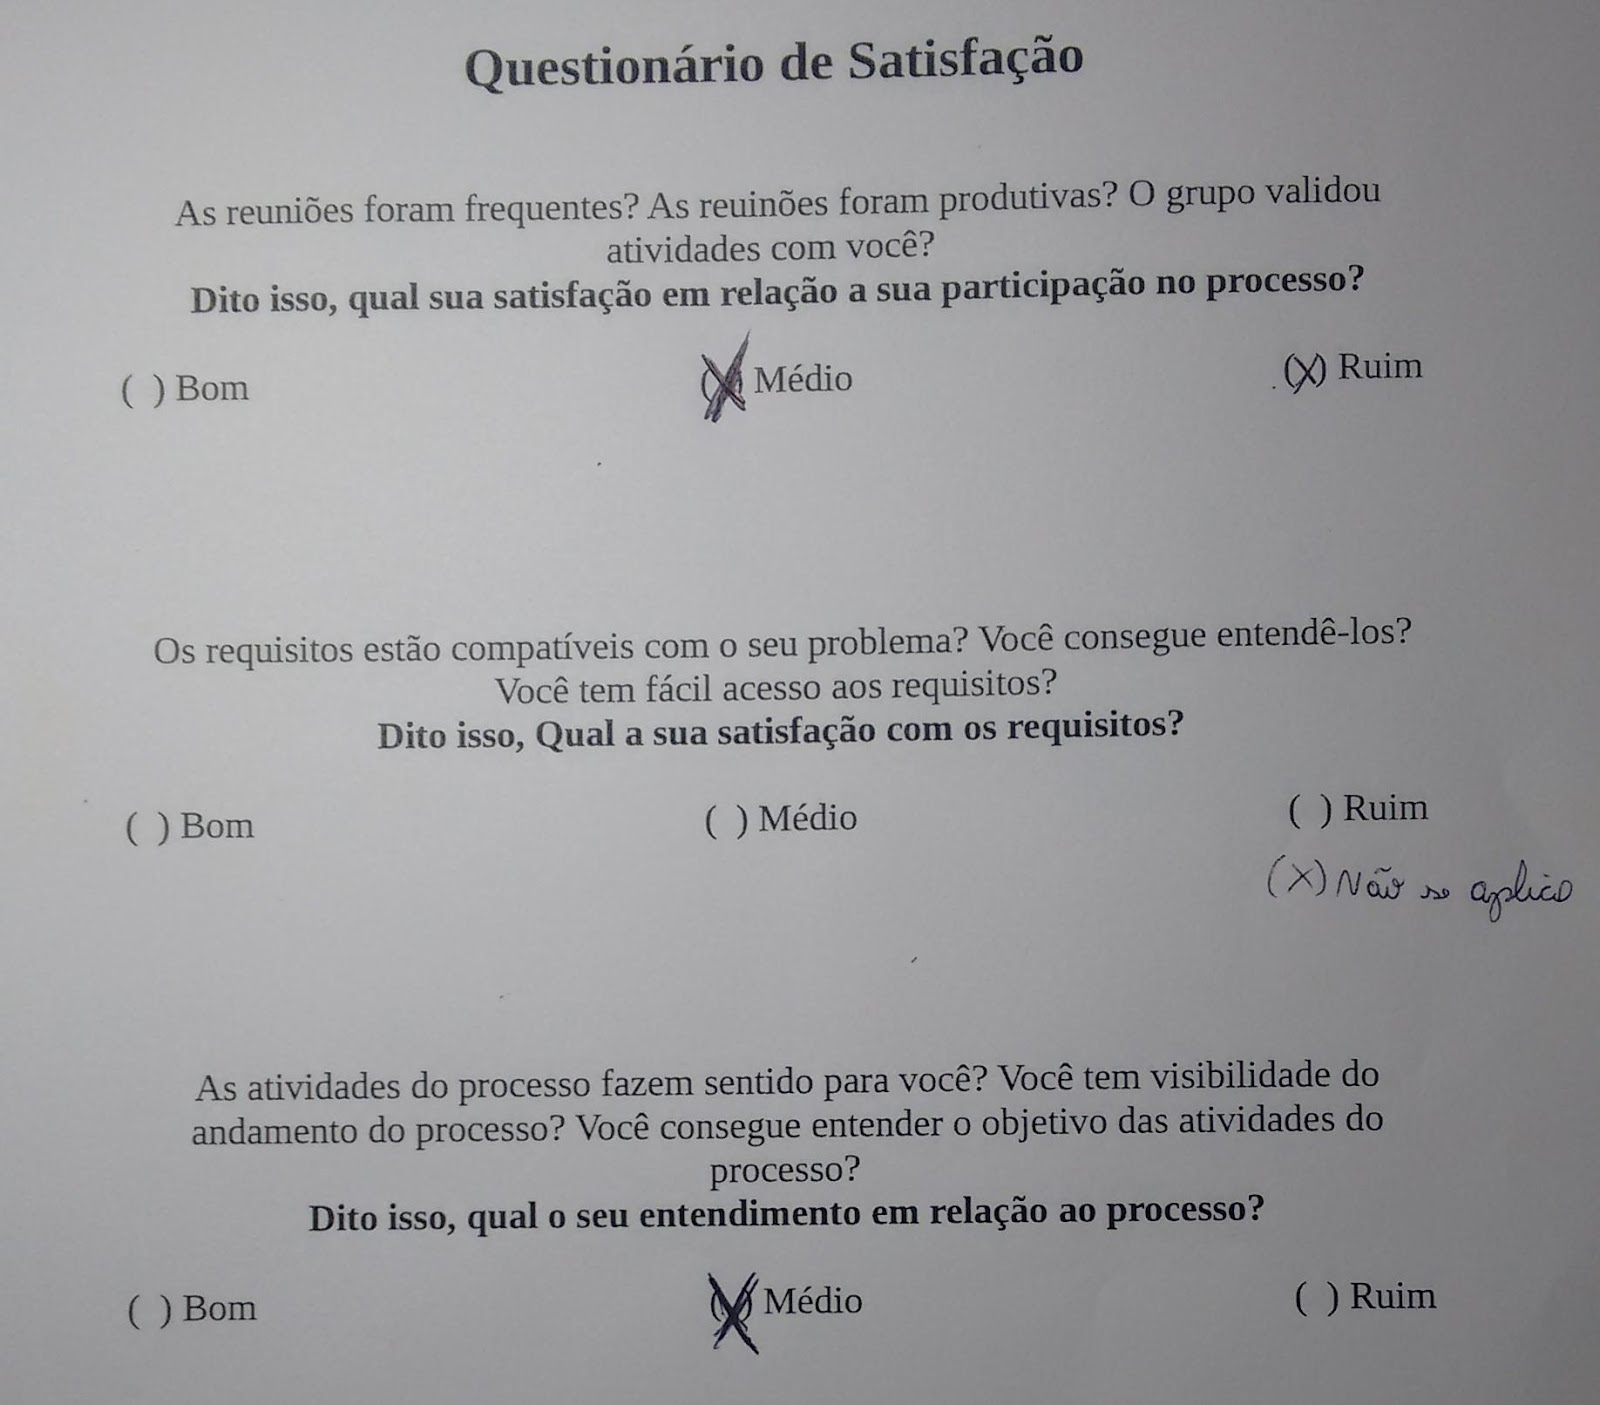
\includegraphics[width=0.8\textwidth]{figuras/quest2}
  \caption{Questionário 1 - Eletrojun}
  \label{fig:quest2}
\end{figure}


\subsection{Conclusão de Iteração}

Pode-se concluir que, a equipe com o contexto da Engrena, que se propuseram a seguir um processo muito mais calcado no modelo de maturidade, tiveram uma base a mais para se orientarem do que o time que teve menos foco e participação no mesmo modelo, e tal ato refletiu na satisfação do cliente.

Tal filosofia também é refletida no esforço da equipe, a qual pode-se observar uma maior dedicação pelo time que mais se apoiou no modelo de maturidade.

Pode-se observar também, que um aumento no orçamento de R\$ 122,40 teria um significativo aumento na produtividade do time, visto que apenas agregando a DRE-01 aumentaria muito os resultados.

\begin{figure}[H]
  \center
  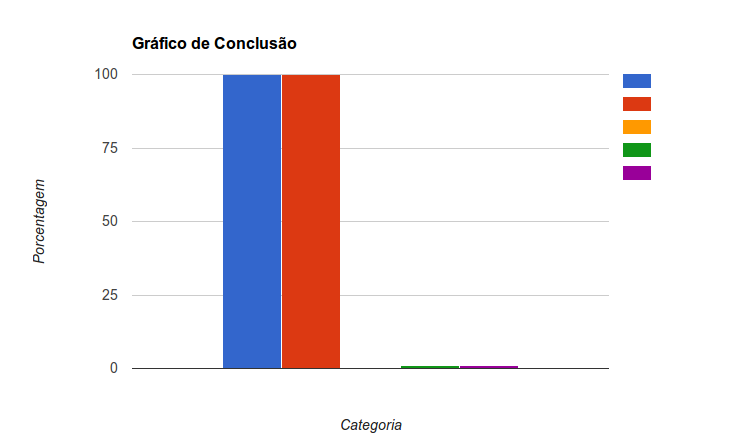
\includegraphics[width=0.8\textwidth]{figuras/plot1}
  \caption{Gráfico de conclusão}
  \label{fig:plot1}
\end{figure}

\section{Iteração 2}

\subsection{Engrena}

\subsubsection{Métricas Coletadas}

\begin{itemize}
\item Esforço da Equipe

\begin{figure}[H]
    \center
    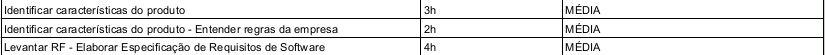
\includegraphics[width=0.8\textwidth]{figuras/esforco-eqp3}
    \caption{Esforço da Equipe - Iteração 2 - Engrena}
    \label{fig:esforco-eqp3}
\end{figure}

\item Esforço dos Monitores

O monitor dedicou-se um total de \textbf{4 horas} nesta iteração em questão.

\item Custo das Atividades

R\$ 550,80

\item Custo de Adesão ao Modelo de Maturidade

DRE-01: R\$ 183,60

DRE-07: R\$ 183,60

GRE-01: R\$ 183,60


\end{itemize}

\subsubsection{Indicadores}

Os indicadores que visamos analisar, para levar em consideração as métricas coletadas são:
\begin{itemize}
\item Satisfação do cliente com os requisitos
\item Satisfação do cliente com o processo
\end{itemize}

Para responder tais, foi elaborado um questionário (figura~\ref{fig:quest3}) e aplicado aos clientes, visando analisar sua satisfação de acordo com os indicadores apresentados acima.

\begin{figure}[H]
  \center
  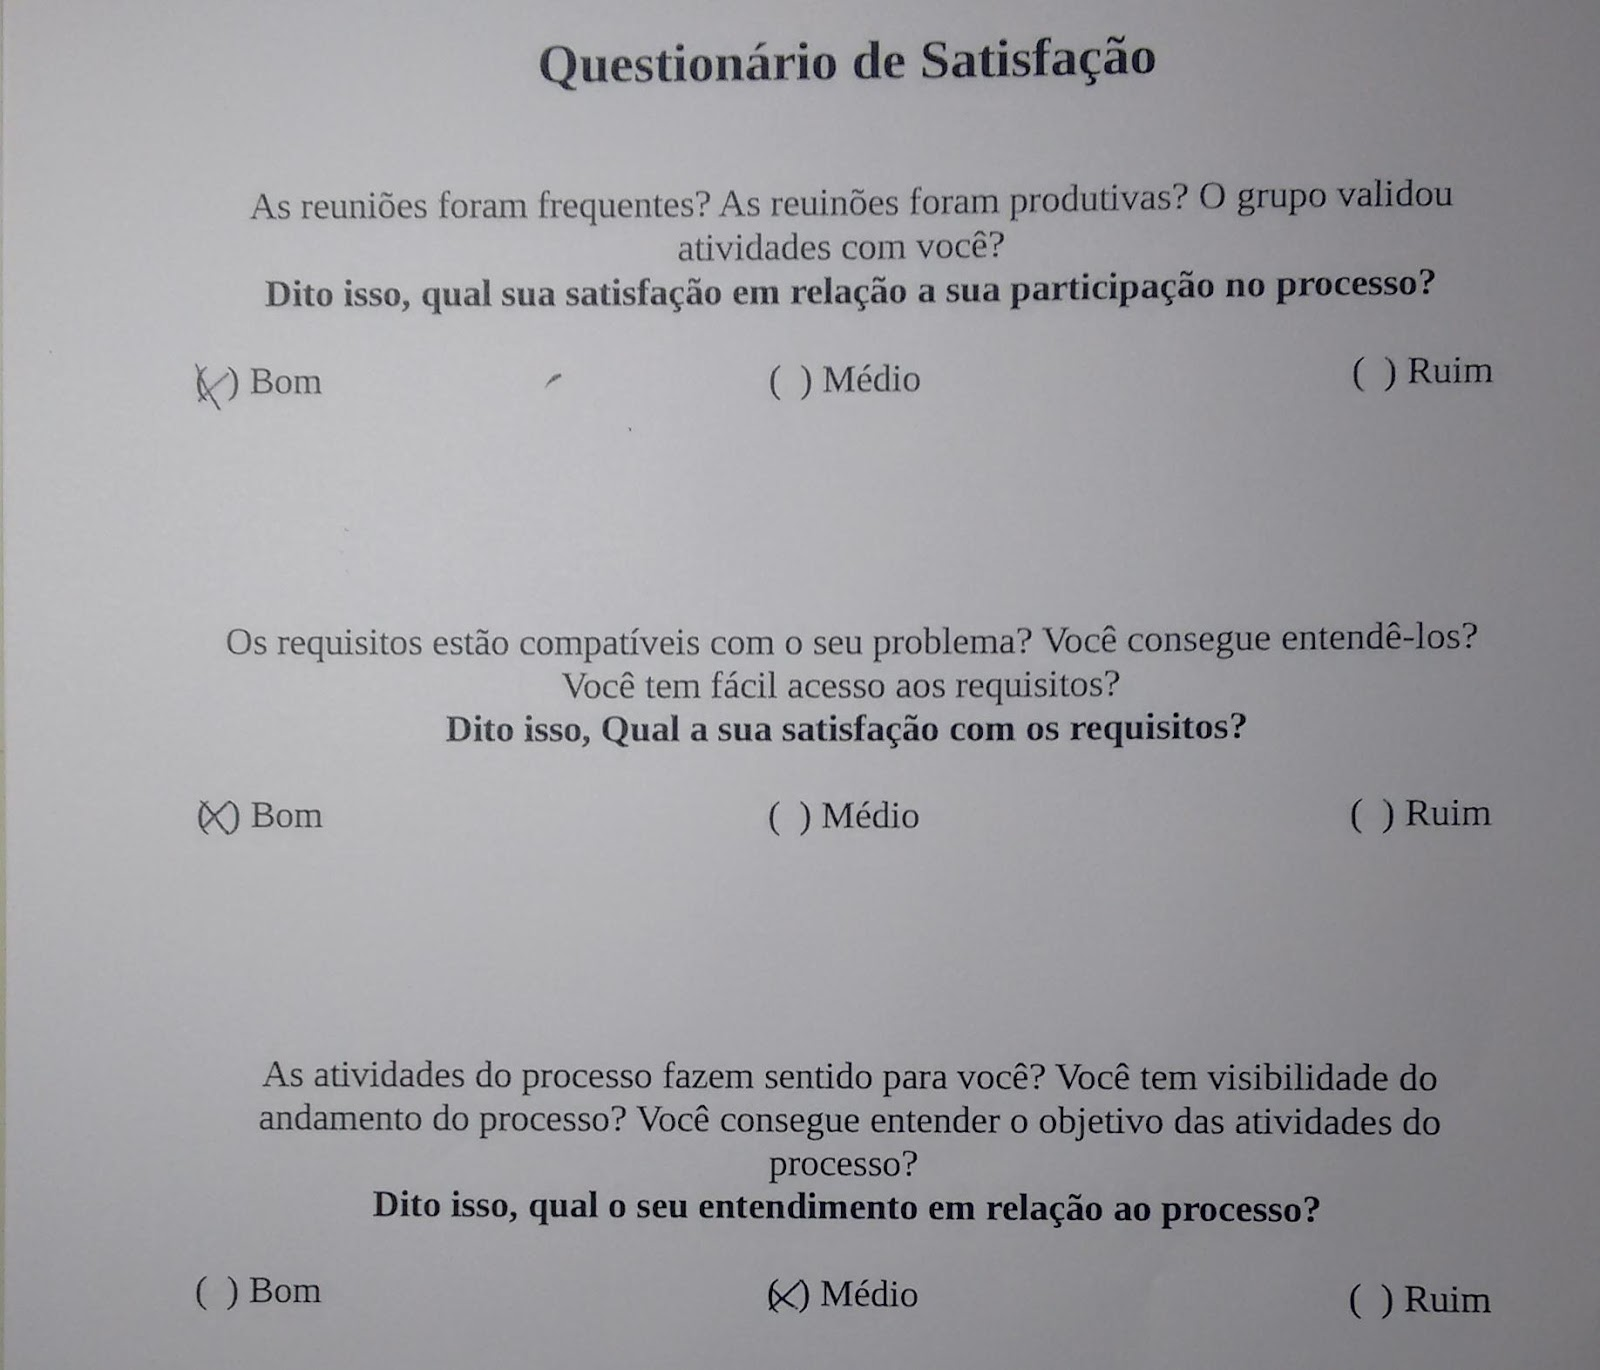
\includegraphics[width=0.7\textwidth]{figuras/quest3}
  \caption{Questionário 2 - Engrena}
  \label{fig:quest3}
\end{figure}

\subsection{Eletrojun}

\subsubsection{Métricas Coletadas}

\begin{itemize}
\item Esforço da Equipe

\begin{figure}[H]
    \center
    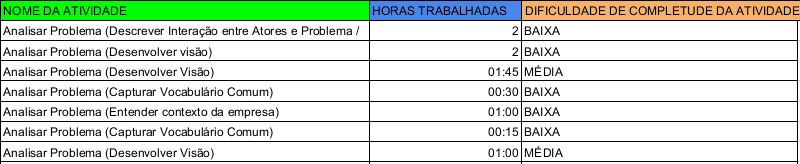
\includegraphics[width=0.8\textwidth]{figuras/esforco-eqp4}
    \caption{Esforço da Equipe - Iteração 2 -Eletrojun}
    \label{fig:esforco-eqp4}
\end{figure}

\item Esforço dos Monitores

O monitor dedicou-se um total de \textbf{4 horas} nesta iteração em questão.

\item Custo das Atividades

R\$ 362,61

\item Custo de Adesão ao Modelo de Maturidade

DRE-01: R\$ 137,70

\end{itemize}

\subsubsection{Indicadores}

Os indicadores que visamos analisar, para levar em consideração as métricas coletadas são:
\begin{itemize}
\item Satisfação do cliente com os requisitos
\item Satisfação do cliente com o processo
\end{itemize}

Para responder tais, foi elaborado um questionário (figura~\ref{fig:quest4}) e aplicado aos clientes, visando analisar sua satisfação de acordo com os indicadores apresentados acima.

\begin{figure}[H]
  \center
  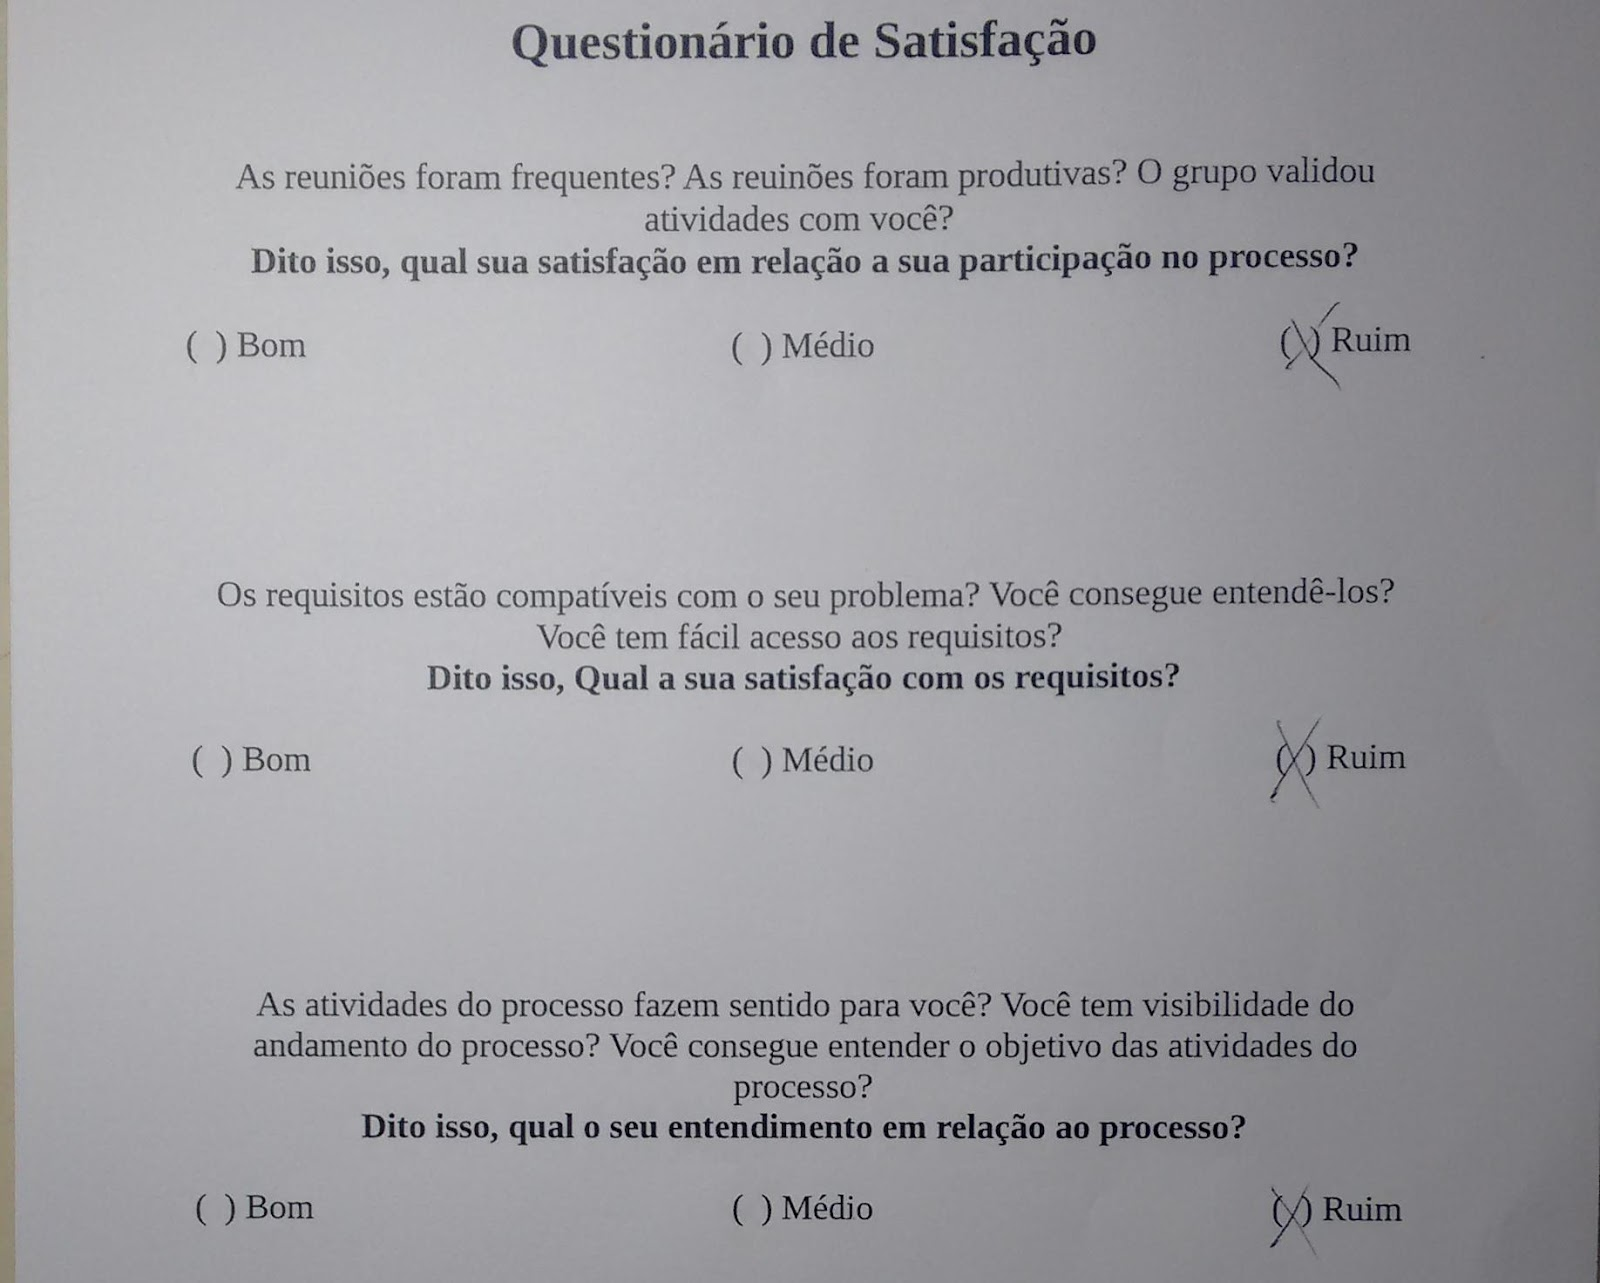
\includegraphics[width=0.8\textwidth]{figuras/quest4}
  \caption{Questionário 2 - Eletrojun}
  \label{fig:quest4}
\end{figure}


\subsection{Conclusão da Iteração}

Pode-se verificar que o grupo da Engrena gastou um previsto de atividades do modelo de maturidade equivalente a R\$ 759,60, enquanto que o outro grupo teve um gasto total de atividades do modelo de maturidade equivalente a R\$ 137,70.

Tendo em vista isso, podemos claramente concluir que tal ação refletiu claramente na satisfação do cliente por parte de diversos fatores, desde o processo até os requisitos.

\begin{figure}[H]
  \center
  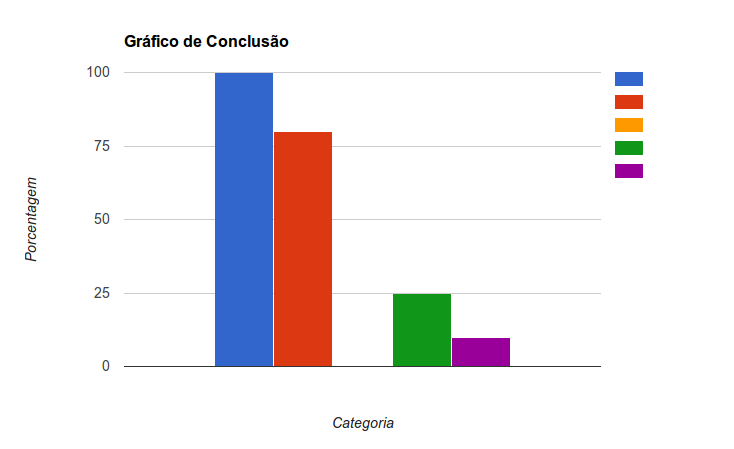
\includegraphics[width=0.8\textwidth]{figuras/plot2}
  \caption{Gráfico de conclusão Iteração 2}
  \label{fig:plot2}
\end{figure}

\section{Iteração 3}

\subsection{Engrena}

\subsubsection{Métricas Coletadas}

\begin{itemize}
\item Esforço da Equipe

\begin{figure}[H]
    \center
    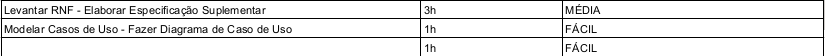
\includegraphics[width=0.8\textwidth]{figuras/esforco-eqp5}
    \caption{Esforço da Equipe - Iteração 3 - Engrena}
    \label{fig:esforco-eqp5}
\end{figure}

\item Esforço dos Monitores

O monitor dedicou-se um total de \textbf{4 horas} nesta iteração em questão.

\item Custo das Atividades

R\$ 306,00

\item Custo de Adesão ao Modelo de Maturidade

DRE-01: R\$ 61,20

DRE-05: R\$ 30,60

DRE-06: R\$ 30,60

DRE-07: R\$ 61,20

GRE-01: R\$ 61,20

\end{itemize}

\subsubsection{Indicadores}

Os indicadores que visamos analisar, para levar em consideração as métricas coletadas são:
\begin{itemize}
\item Satisfação do cliente com os requisitos
\item Satisfação do cliente com o processo
\end{itemize}

Para responder tais, foi elaborado um questionário (figura~\ref{fig:quest5}) e aplicado aos clientes, visando analisar sua satisfação de acordo com os indicadores apresentados acima.

\begin{figure}[H]
  \center
  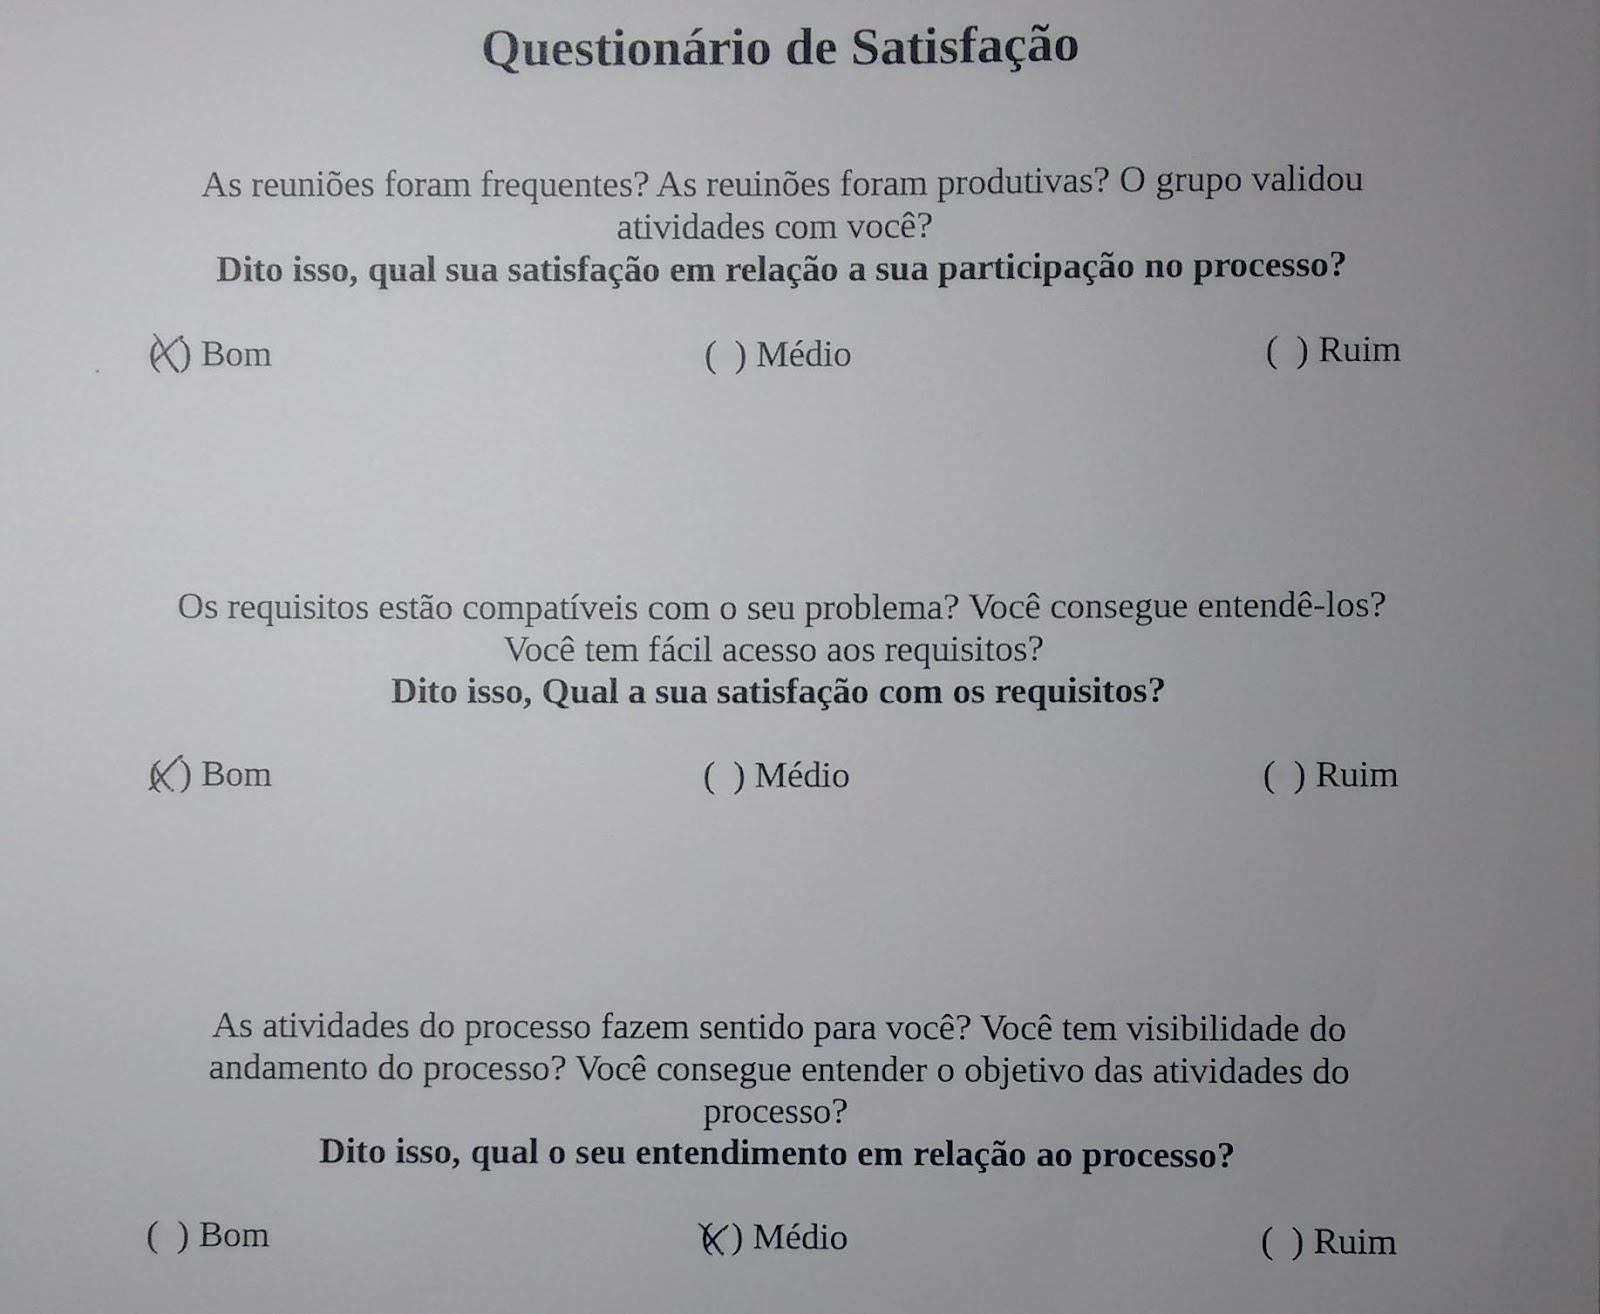
\includegraphics[width=0.7\textwidth]{figuras/quest5}
  \caption{Questionário 3 - Engrena}
  \label{fig:quest5}
\end{figure}

\subsection{Eletrojun}

\subsubsection{Métricas Coletadas}

\begin{itemize}
\item Esforço da Equipe

\begin{figure}[H]
    \center
    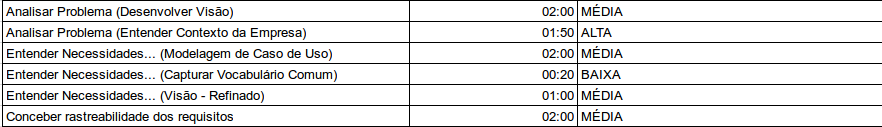
\includegraphics[width=0.8\textwidth]{figuras/esforco-eqp6}
    \caption{Esforço da Equipe - Iteração 3 Eletrojun}
    \label{fig:esforco-eqp6}
\end{figure}

\item Esforço dos Monitores

O monitor dedicou-se um total de \textbf{4 horas} nesta iteração em questão.

\item Custo das Atividades

R\$ 399,33

\item Custo de Adesão ao Modelo de Maturidade

DRE-01: R\$ 68,85

DRE-05: R\$ 45,90

GRE-06: R\$ 45,90

\end{itemize}

\subsubsection{Indicadores}

Os indicadores que visamos analisar, para levar em consideração as métricas coletadas são:
\begin{itemize}
\item Satisfação do cliente com os requisitos
\item Satisfação do cliente com o processo
\end{itemize}

Para responder tais, foi elaborado um questionário (figura~\ref{fig:quest6}) e aplicado aos clientes, visando analisar sua satisfação de acordo com os indicadores apresentados acima.

\begin{figure}[H]
  \center
  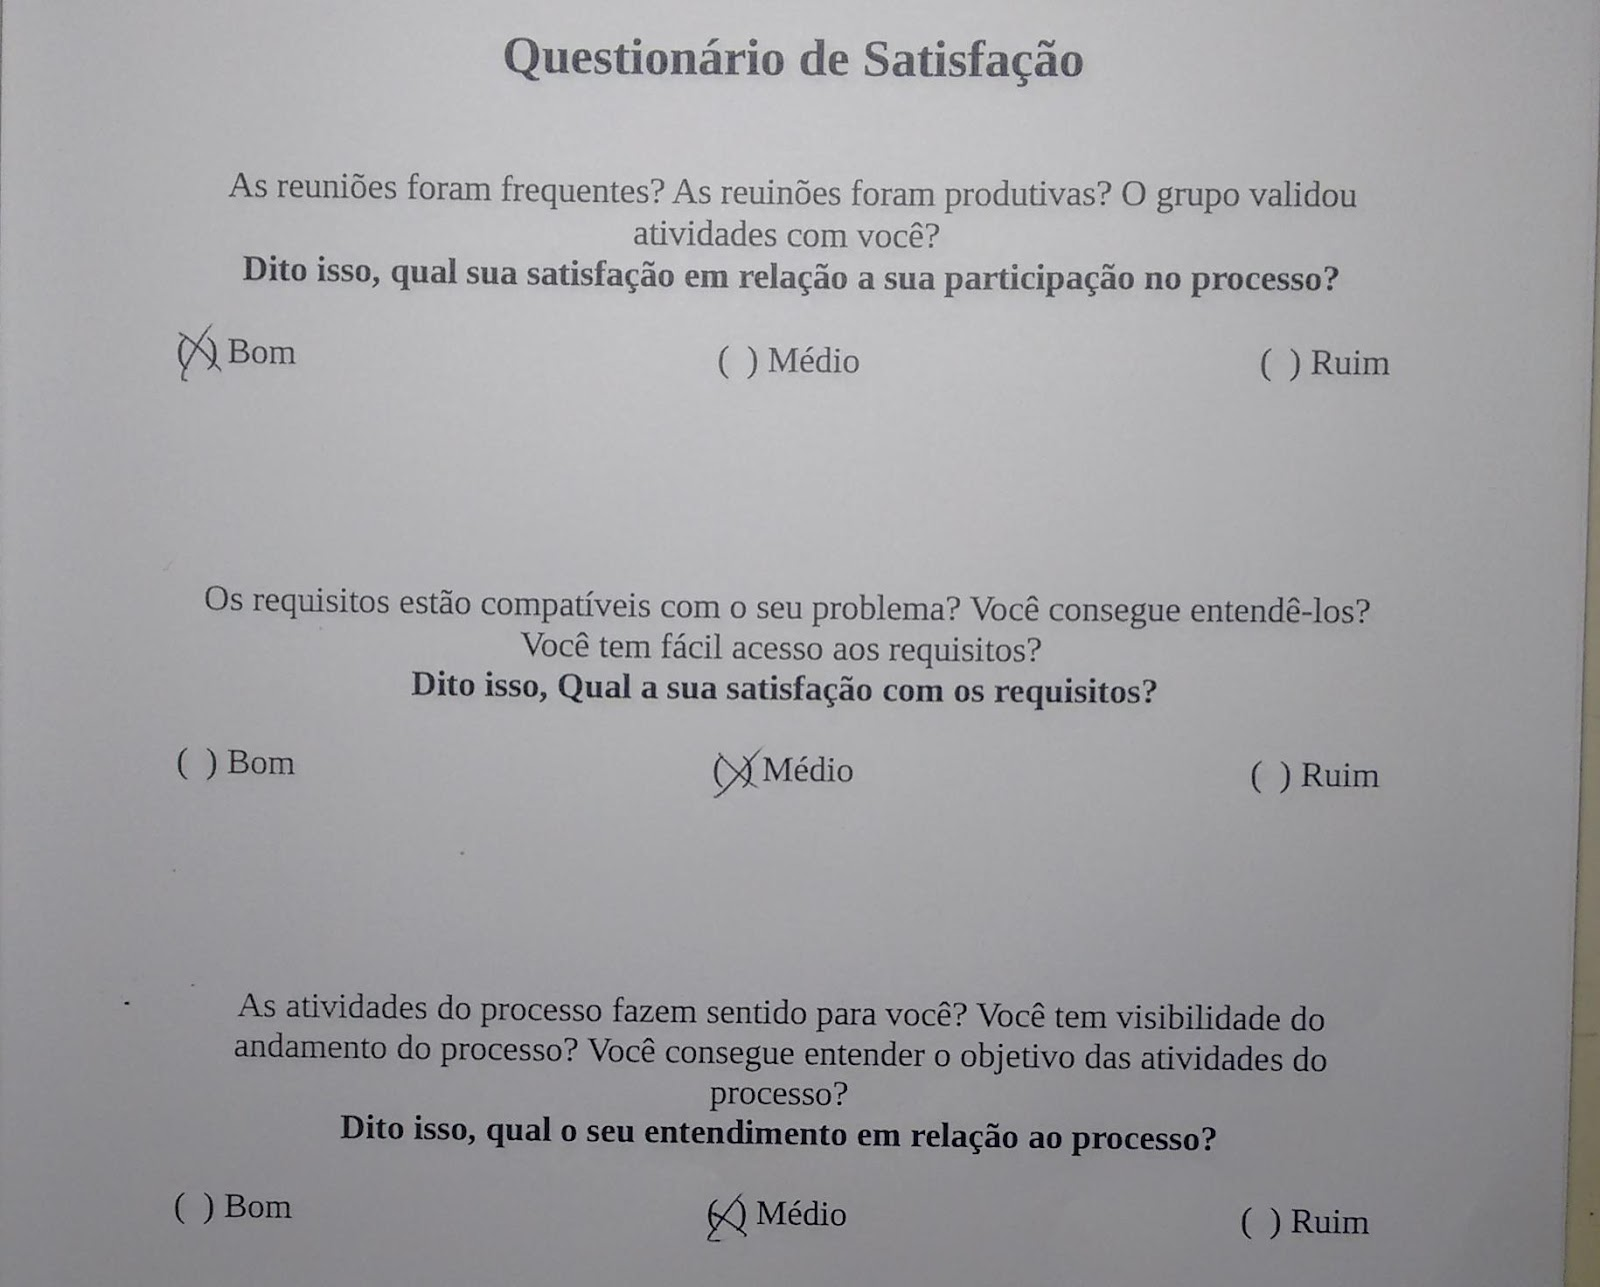
\includegraphics[width=0.8\textwidth]{figuras/quest6}
  \caption{Questionário 3 - Eletrojun}
  \label{fig:quest6}
\end{figure}


\subsection{Conclusão da Iteração}

Mais uma vez, pode-se ver que o grupo do contexto da Engrena, ao se apoiar mais no modelo de maturidade, teve-se um sucesso maior ao lidar com a satisfação do cliente.
O grupo da Engrena, investiu um total de R\$ 244,80 em atividades do MPS-Br, já o grupo da Eletrojun investiu um total de R\$ 160,65, sendo esse investimento, mais uma vez, refletido na satisfação de seus clientes.
Logo, abaixo pode-se ver o gráfico da comparação da quantidade aderida de um modelo de maturidade contra a satisfação do cliente, entre os dois grupos.

\begin{figure}[H]
  \center
  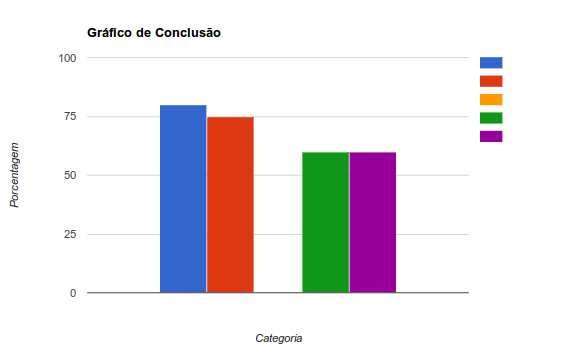
\includegraphics[width=0.8\textwidth]{figuras/plot3}
  \caption{Gráfico de conclusão Iteração 3}
  \label{fig:plot3}
\end{figure}


\section{Iteração 4}

Devido ao prazo de entrega deste relatório, e pelos grupos analisados 
ainda não terem iniciados as atividades previstas para essa iteração, 
\textbf{a iteração 04 não será englobada}, apesar de prevista.

Apesar de tal imprevisto, ainda foi possível analisar a satisfação dos clientes neste intervalo. Abaixo está explicito tais resultados.

\begin{figure}[H]
  \center
  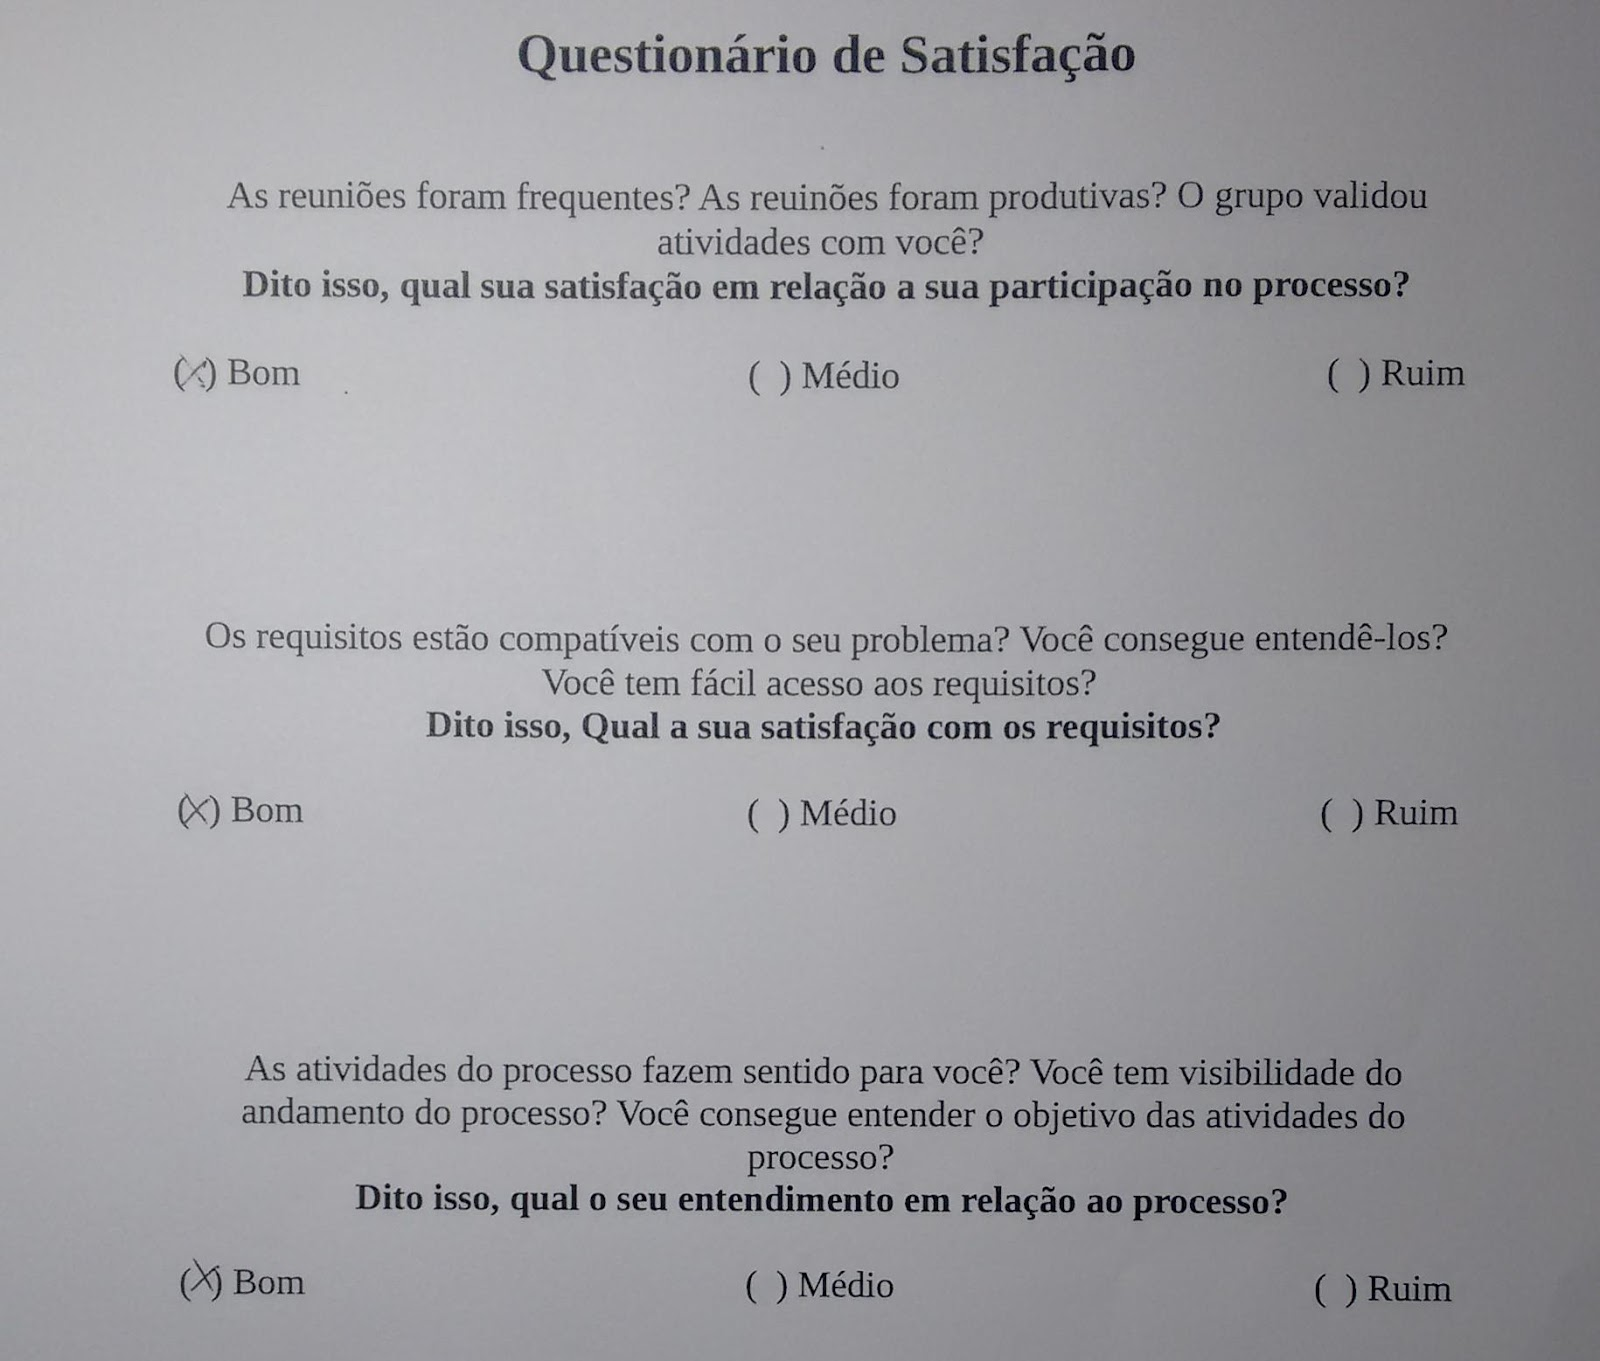
\includegraphics[width=0.7\textwidth]{figuras/quest7}
  \caption{Questionário 4 - Engrena}
  \label{fig:quest7}
\end{figure}

\begin{figure}[H]
  \center
  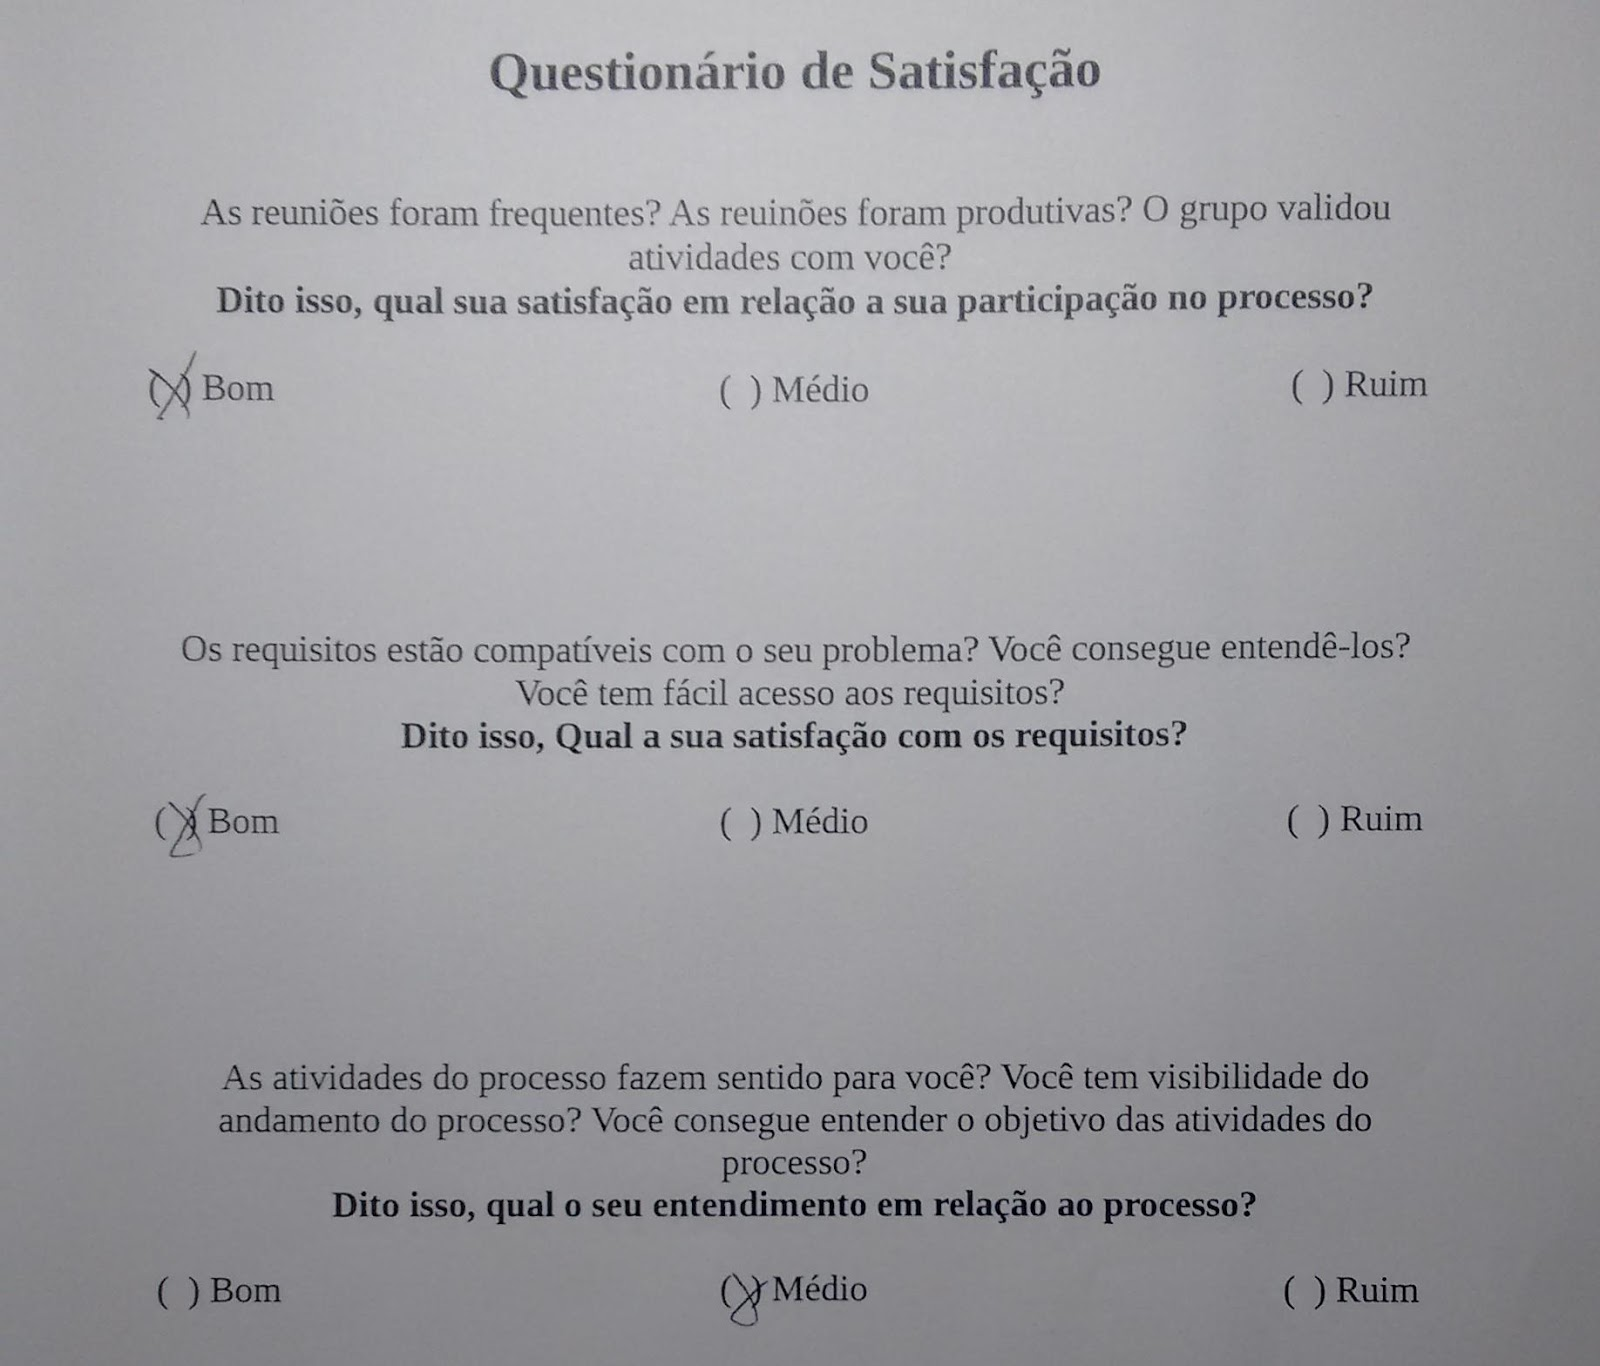
\includegraphics[width=0.7\textwidth]{figuras/quest8}
  \caption{Questionário 4 - Eletrojun}
  \label{fig:quest8}
\end{figure}


